	
	Soit $f$ la fonction définie sur $[0 ; +\infty[$ par :
	\[
	f(x) = -x^2 + 2x + 4.
	\]
	Dans le plan muni d'un repère orthonormé, on note $C$ sa courbe représentative.
	
	\subsection*{Question 1}
	
	La fonction $f$ est dérivable sur $\mathbb{R}$, donc en particulier sur $[0 ; +\infty[$. Calculons sa dérivée :
	\[
	f'(x) = -2x + 2 = 2(1 - x).
	\]
	
	Étudions le signe de $f'(x)$ :
	\begin{itemize}
		\item $f'(x) > 0$ si $1 - x > 0$, soit $x < 1$ : la fonction $f$ est donc croissante sur $[0 ; 1]$ ;
		\item $f'(x) < 0$ si $1 - x < 0$, soit $x > 1$ : la fonction $f$ est décroissante sur $[1 ; +\infty[$ ;
		\item $f'(x) = 0$ si $1 - x = 0$, soit $x = 1$.
	\end{itemize}
	\begin{center}
		\begin{tikzpicture}
			\tkzTabInit[lgt=3, espcl=3]
			{$x$/1, $f'(x)$/1, $f(x)$/2}
			{$0$, $1$, $+\infty$}
			\tkzTabLine{,+,z,-}
			\tkzTabVar{-/$4$, +/$5$, -/}
		\end{tikzpicture}
	\end{center}
	On a donc un maximum local en $x = 1$ :
	\[
	f(1) = -(1)^2 + 2 \times 1 + 4 = 5.
	\]
	Le maximum de la fonction $f$ sur $[0 ; +\infty[$ est donc $f(1) = 5$.
	
	\subsection*{Question 2}
	
	Cherchons les points d'intersection de $C$ avec l'axe des abscisses, c'est-à-dire les solutions de l'équation $f(x) = 0$ :
	\[
	-x^2 + 2x + 4 = 0.
	\]
	
	Calculons le discriminant :
	\[
	\Delta = 2^2 - 4 \times (-1) \times 4 = 4 + 16 = 20.
	\]
	Comme $\Delta > 0$, l'équation admet deux solutions réelles :
	\[
	x_1 = \frac{-2 - \sqrt{20}}{-2}, \quad x_2 = \frac{-2 + \sqrt{20}}{-2}.
	\]
	La première racine, $x_1$, est négative, donc seule $x_2 = 1 + \sqrt{5}$ est valable dans l'intervalle $[0 ; +\infty[$.\\
	Le point d'intersection $A$ a donc pour coordonnées $(1 + \sqrt{5} ; 0)$.
	
	\subsection*{Question 3}
	
	L'équation réduite de la tangente $T$ à la courbe $C$ au point d'abscisse $2$ est donnée par :
	\[
	y - f(2) = f'(2)(x - 2).
	\]
	Calculons $f(2)$ et $f'(2)$ :
	\[
	f(2) = -(2)^2 + 2 \times 2 + 4 = 4, \quad f'(2) = 2 \times (1 - 2) = -2.
	\]
	L'équation de la tangente est donc :
	\[
	y - 4 = -2(x - 2) \quad \text{soit} \quad y = -2x + 8.
	\]
	
	\subsection*{Question 4}
	
	Voici une représentation schématique de la courbe $C$ et de sa tangente en $x = 2$ :
\begin{center}
	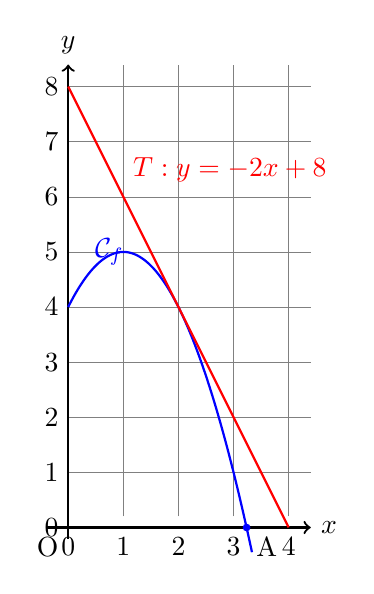
\begin{tikzpicture}[scale=0.7]
	% Grille
	\foreach \x in {0,1,...,4} {
		\draw[very thin, gray] (\x, 0.2) -- (\x, 8.4);
		\node[below] at (\x, 0) {\x};  % Valeurs sur l'axe des x
	}
	\foreach \y in {0,1,...,8} {
		\draw[very thin, gray] (0, \y) -- (4.4, \y);
		\node[left] at (0, \y) {\y};  % Valeurs sur l'axe des y
	}
	
	% Axes
	\draw[thick,->] (-0.4, 0) -- (4.4, 0) node[right] {$x$};
	\draw[thick,->] (0, -0.2) -- (0, 8.4) node[above] {$y$};
	
	% Fonction f(x)
	\draw[domain=0:3.3361, samples=200, smooth, thick, blue] plot (\x, {(\x)*(\x)*(-1) + 2*(\x) + 4});
	
	% Droite T : y = -2x + 8 (en rouge)
	\draw[domain=0:4, samples=200, smooth, thick, red] plot (\x, {-2*\x + 8}) ;
		\node[right,red] at (1,6.5) {$T : y = -2x + 8$};
	% Points
	\node[below right] at (3.2361,0) {A};
	\fill[blue] (3.2361, 0) circle (2pt);
	\node[below left] at (0, 0) {O};
	
	% Label courbe
	\node[blue] at (0.75, 5) {$\mathcal{C}_f$};
\end{tikzpicture}
\end{center}

	

	
	
